Modalitatea prin care componentele crawler-ului web "Surf" pot fi accesate, modificate și executate este reprezentată de o interfață\cite{iterface-definition} structurată sub forma unui API RESTful\footnote{engl. \textit{RESTful} = adjectiv de la abrevierea \textit{REST}; un API este \textit{RESTful} dacă adoptă stilul arhitectural \textit{REST\cite{rest-definition}}}. API-ul adoptă stilul arhitectural REST\cite{rest-definition} deoarece acesta ajută la decuplarea arhitecturii și simplificarea urmăririi executiei aplicației, prin faptul că nu permite memorarea stărilor intermediare în cadrul unei sesiuni de comunicare între utilizator ți crawler. De asemenea, API-ul RESTful conferă extensibilitate și flexibilitate la nivel de interfață, întrucât permite gruparea resurselor în mod ierarhic și identificarea ușoară a resurselor și a consecințelor aplicării anumitor acțiuni, prin verbe HTTP, asupra stării sistemului. \textit{Figura 8} prezintă secvența mimimă de operații ce trebuie efectuate, la nivel de API, pentru a putea obține rezultate în urma procesului de parcurgere a paginilor web de catre crawler, modelate printr-o diagramă de secvență.

% Locatie creare diagrama secventa: http://gojs.net/latest/samples/sequenceDiagram.html
% Script creare diagrama secventa:
\iffalse
{ "class": "go.GraphLinksModel",
  "nodeDataArray": [
{"key":"User", "text":"Utilizator", "isGroup":true, "loc":"0 0", "duration":19},
{"key":"Api", "text":"API-ul 'Surf'", "isGroup":true, "loc":"250 0", "duration":19},
{"key":"Backend", "text":"Backend AWS", "isGroup":true, "loc":"500 0", "duration":19},
{"group":"User", "start":1, "duration":4},
{"group":"Api", "start":1, "duration":3},
{"group":"Backend", "start":2, "duration":2},
{"group":"User", "start":6, "duration":4},
{"group":"Api", "start":6, "duration":3},
{"group":"Backend", "start":7, "duration":2},
{"group":"User", "start":11, "duration":4},
{"group":"Api", "start":11, "duration":3},
{"group":"Backend", "start":12, "duration":2},
{"group":"User", "start":16, "duration":4},
{"group":"Api", "start":16, "duration":3},
{"group":"Backend", "start":17, "duration":2}
 ],
  "linkDataArray": [
{"from":"User", "to":"Api", "text":"POST /workflows", "time":1},
{"from":"Api", "to":"Backend", "text":"Validare & înregistrare workflow", "time":2},
{"from":"Backend", "to":"Api", "text":"Workflow din baza de date :id_workflow", "time":3},
{"from":"Api", "to":"User", "text":"Workflow din baza de date :id_workflow", "time":4},
{"from":"User", "to":"Api", "text":"POST /workflows/executions :id_workflow", "time":6},
{"from":"Api", "to":"Backend", "text":"Pornește workflow", "time":7},
{"from":"Backend", "to":"Api", "text":"Execuție cu id :id_executie", "time":8},
{"from":"Api", "to":"User", "text":"Execuție cu id :id_executie", "time":9},
{"from":"User", "to":"Api", "text":"GET /workflows/executions/:id_executie", "time":11},
{"from":"Api", "to":"Backend", "text":"Listează execuție", "time":12},
{"from":"Backend", "to":"Api", "text":"Detalii execuție", "time":13},
{"from":"Api", "to":"User", "text":"Detalii execuție", "time":14},
{"from":"User", "to":"Api", "text":"GET /workflows/executions/:id_executie/metadata", "time":16},
{"from":"Api", "to":"Backend", "text":"Listează metadatele asociate execuției :id_executie", "time":17},
{"from":"Backend", "to":"Api", "text":"Metadate asociate cu :id_executie", "time":18},
{"from":"Api", "to":"User", "text":"Metadate asociate cu :id_executie", "time":19}
 ]}
\fi

\begin{figure}[ht]
\begin{center}
	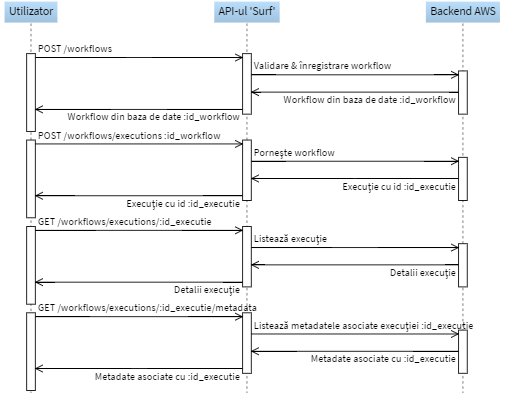
\includegraphics[keepaspectratio, width=0.9\textwidth]{diagrama-utilizator-api.png}
	\caption{Interacțiunea utilizator - API \cite{diagram-icons-sources, aws-icons-source}}\par\medskip 

\end{center}
\end{figure}

\noindent
API-ul construit este securizat suplimentar, în afara drepturilor de acces stabilite prin rolurile IAM, prin necesitatea deținerii unei chei de acces de către utilizatorul acestuia. Cheile de acces se creează programatic, de către generatorul de resurse, și au, fiecare, asociate, politici de restricție a utilizării API-ului. Politicile de restricție constau în limitări impuse de către sistemul cloud asupra ratei la care se accesează API-ul, folosind o anumită cheie de acces. Există doua categorii de limitări în ceea ce privește controlul traficului autentificat asupra API-ului "Surf", conform algoritmului \textit{token bucket}:

\begin{itemize}
	\item{\textit{Limitarea ratei de acces regulat:} se referă la controlarea numărului maxim de cereri pe secundă pe care un utilizator autentificat le poate face în mod normal;}
	
	\item{\textit{Limitarea ratei de acces în cascadă\footnote{engl. \textit{burst limit}}:} se referă la controlarea cantității extraordinare de cereri care pot surveni ca răspuns la un anumit eveniment extern (e.g. mai multe workflow-uri sunt pornite la o anumită oră din zi).}
	
\end{itemize}